\documentclass{mcmthesis}
\mcmsetup{CTeX = true,
        tcn = 83451, problem = A,
        sheet = true, titleinsheet = true, keywordsinsheet = true,
        titlepage = false, abstract = false}
\usepackage{palatino}
\usepackage{graphicx}
\usepackage{url}
\title{ The solve of MCM 2018 problem A }
\author{\small Team \# 83451}
\date{\today}
\begin{document}

\begin{abstract}

waiting to add!

\begin{keywords}
  Try; Table; Picture; Reference
\end{keywords}
\end{abstract}
\maketitle

\tableofcontents
\newpage

\section{Introduction}

\subsection{Motivation}

On a sunny summer day, everyone wants to enjoy the pleasure of fishing on a yacht at sea. However, as we enter the deep ocean, chances are that our on-board HF(3-30MHz) receiver was unable to receive timely broadcast warnings of the coming bad weather from the Maritime Bureau, then our wonderful summer afternoon would be destroyed by the ensuing storm. Based on the current HF broadcast model, which consists a blind area, such stories will be staged on the sea for many years.

\subsection{Problem Restatement}


\section{General Assumptions}

    To simplify the real life situation, we will accept the following assumptions while we construct our models.

    \begin{itemize}

      \item a. We assume that the transmitting antenna radiates a particular frequency of spherical waves.

      \item b. According to the far propagating distance, the Earth-surface cannot be considered as a plane, which we always do to handle some daily problems. However, we can approximate the Earth  to a sphere with a radius of 640,000 km. In addition, \textbf{the ionosphere and the ocean are in concentric spheres}.

      \item c. Due to the facts that the light wave is one kind of \textbf{electromagnetic waves (EM waves)}, we assume that the ionosphere and the ocean’s reflection of EM waves can be analyzed using the same method as \textbf{geometrical optics}.

      \item d. Suppose the temperature and pressure in the entire propagation space path are almost constant, which means we will ignore the loss of EM waves caused by flowing air or non-constant physical characters (especially the temperature and pressure).

      \item e. We will not justify the electromagnetic noise from the radio receiver. We will assume that the noise mainly comes from the atmosphere.

    \end{itemize}

\section{Constants and Notations}

    In order to calculate and describe our mathematical model more simply and clearly, we will use the following mathematical notation, where the values we assume or determine as constants will give its values and units here in Table \ref{tab:Constants}. Some of the units such as \emph{$dB$ and $dBm$} is not easy to see in other field. The details of these less commonly used units will be discussed later.

    \begin{table}[h]
      \centering
        \begin{tabular}{|c|c|c|}

          \hline Constants & Definition & Value (with units) \\
          \hline $P_{initial}$ & How much energy does the initial HF signal has & $100(W)$ \\
          \hline

        \end{tabular}
        \caption{Constants}
        \label{tab:Constants}
    \end{table}


    \begin{table}[h]
      \centering
        \begin{tabular}{|c|c|l|}

          \hline Notations & Definition & Unit \\
          \hline $E_{r}$ & How much energy may trasmit to the receiver & $dBm$ \\
          \hline $E_{g}$ & How much energy will be generated & $dBm$ \\
          \hline $G_{r}$ & The antennas gain of receiver & $dBi$ \\
          \hline $G_{g}$ & The antennas gain of generator & $dBi$ \\
          \hline $L_{totle}$ & The totle energy loss during the propagation & $dB$ \\
          \hline $L_{fspl}$ & The free space path loss & $dB$ \\
          \hline $L_{a}$ & The loss during passing the ionosphere layer & $dB$ \\
          \hline $L_{gd}$ & The loss during the reflection on the grond & $dB$ \\
          \hline $L_{addition}$ & Additional loss of the signal energy & $dB$ \\
          \hline

        \end{tabular}
        \caption{Notations}
    		\label{tab:Notations}
    \end{table}



\section{The High Frequency Electromagnetic Waves}
  \subsection{The High Frequency Electromagnetic Waves (HF-EM waves).}

    The electromagnetic wave, in physics, refers to the wave of the electronic field, propagating through space-time, carrying electromagnetic radiant energy. Classically, we can just study one component of the electromagnetic wave to represent the physical state of the entire wave. And the EM waves can be described as:

      \begin{equation}\label{eq:EMW}
        E = A * \cos(\omega t + \phi_{0})
      \end{equation}
      Where: \\
      $E$ is represent the electric field strength; \\
      $\omega$ is the angular frequency;\\
      $t$ represents how much time has passed since the wave had been generated;\\
      $\phi_{0}$ is the initial phase of the wave.\\

      As we known, \textbf{high frequency (HF)} is the designation for the range of radio frequency EM waves between 3 and 30 megahertz (MHz). The most interesting and important property of this frequency band, is that it can be reflected in the ionosphere layer in the atmosphere — a method which named \emph{sky wave} or \emph{skip}. It is because that the ionized atoms in the atmosphere can interact with HF-EM waves to change its radiating path.\cite{HF_EM}

      If the sky wave which reflected to the Earth can be reflected again by the ground, a \emph{multi-hop propagation} model would be formed between the ionosphere and the Earth-surface(Figure ~\ref{fig:Multi_hop}). Depending on multi-hop propagation, the scope of the HF communications has been greatly enhenced.

      \begin{figure}[ht]
      \centering
      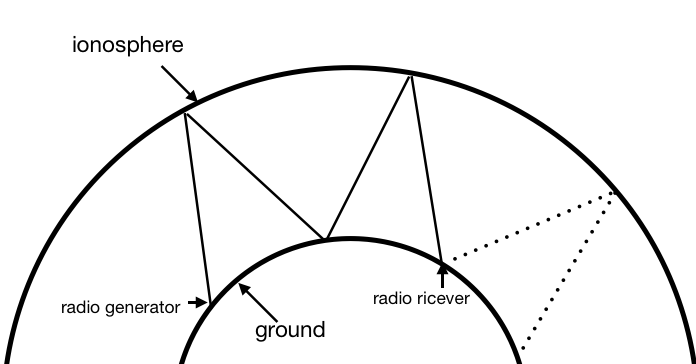
\includegraphics[scale=0.5]{Multi_hop}
      \caption{The Multi-hop propagation}
      \label{fig:Multi_hop}
      \end{figure}


  \subsection{HF-EM waves Propagation Model}

    Based on the modern physics common knowledge, HF-EM waves use the energy of the electromagnetic field to transmit information. So we can determine the signal strength by simply considering its enery. Especially in the radio-related applications, we usually use the unit known as decibel(\emph{dB}) to represent the energy relation of radio wave generating, transmitting and receiving. The decibel is a logarithmic unit used to express the ratio of the physical property to another, and may be used to describe a change in the value we discussed. Normally, the method of using decibel to describe the power quantity is:

      \begin{equation}\label{eq:power_dB}
        N|_{dB} = 10 \lg(\frac{P_{i}|_{W}}{P_{0}|_{W}})
      \end{equation}
      Where: \\
      $N$ represents the decibel figure we need to describe the ratio of the \textbf{current power} $P_{i}$ to the \textbf{initial power} $P_{0}$.\\

    In this paper, we will adopt this unit to describe the loss of the power in both of the ionosphere and ocean surface. Since we are solving a radio-related issue, to simplify our calculation, we will also use a unit named as dBm (power relative to 1 milliWatt) to measure the power of our EM waves. By the Equation \ref{eq:power_dB}, we get:

      \begin{equation}\label{eq:dBm_milliWatt}
        E |_{dBm} = 10 \lg(\frac{P_{i}|_{W}}{1 |_{mW} })
      \end{equation}

    Because we always use $W(Watt)$ as the power units, so the following Equation is commonly used:

      \begin{equation}\label{eq:dBm_Watt}
        E |_{dBm} = 30 + 10 \lg(\frac{P_{i}|_{W}}{1 |_{W} })
      \end{equation}

    In order to simulate the performance of multi-hop HF-EM waves between the ionosphere and the ocean, we need to measure the physical condition of it. As a EM wave, the essential property is how much energy it has. So the rate of its energy loss is the key factor in accessing a signal propagation process. Using the derived Equation \ref{eq:dBm_Watt} and the unit(dB), the rate of the energy loss can be calculate like this:

      \begin{equation}\label{eq:transmitting}
        E_{r} = E_{g} + G_{g} - L_{totle} + G_{r}
      \end{equation}
      The characters we used has been discussed at Table \ref{tab:Notations}. Since the units \emph{$dBi$} and \emph{$dBm$} has the same meaning of \emph{$dB$}, we can put them together in one formular. The physics meaning of this Equation is easy to understand. As the \emph{$dB$} represents the logarithmic ratio of two number, the multiplications between the initial energy values and the ratios of gain and attenuation can be simply replaced by addition and subtraction.

    From the requirement, which directly give us the energy intensity($P_{initial} = 100 W $) of the initial EM wave, we can assume that the initial wave energy containing both of the generating energy and the gain. Then, using Equation \ref{eq:dBm_Watt}, we can get this result:

      \begin{equation}\label{eq:E_initial}
        E_{initial} = E_{g} + G_{g} = 50 (dBm)
      \end{equation}

    As for the loss of the enery $L_{totle}$, we assume the components of it are:

      \begin{equation}
        L_{totle} = L_{fspl} + L_{a} + L_{gd} + L_{addition}
      \end{equation}

     In this section, we will only study on the free-space path loss ($L_{fspl}$). And the details of other sections of the enery loss will be analyzed later.

  \subsection{The Free-space Path Loss}

      The \textbf{ree-space path loss(FSPL)}\cite{freespacepathloss} has been discussed for many years. FSPL can be used to calculate the signal strength loss when an EM wave travels over a line of sight path in free space. Based on the \emph{Assumption a} and exsting model of spherical waves in free space \emph{(between the ionosphere and the ground)}, we can draw the result of that:

        \begin{equation}\label{eq:FSPL_old}
          L_{fspl} = (\frac{4 \pi d f}{c})^{2}
        \end{equation}
        Where: \\
        $d$ is the distance of the receiver from the transmitter (metres)\\
        $f$ is the signal frequency (Hertz)\\
        $c$ is the speed of light in a vacuum (metres per second)\\

      If we use \emph{dB} as the unit, then we convert this formula to:

        \begin{equation}\label{eq:FSPL_applied}
          L_{fspl} = 20\log(d) + 20\log(f) + 32.44
        \end{equation}
        Where:\\
        $d$ is the distance of the receiver from the transmitter (km)\\
        $f$ is the signal frequency (MHz)\\

      \emph{Notice: the units we use in the Equation \ref{eq:FSPL_old} and Equation \ref{eq:FSPL_applied} are different.}

      By applying this formular, the FSPL can be simply calculated if we have the value of free space distance and the frequency of our EM wave.

\section{The Ionosphere}

  \subsection{The Ionosphere Structure Model}
    The ionosphere is a shell of electrons and electrically charged atoms and molecules that surrounds the Earth, stretching from a height of about 50 km to more than 1,000 km. It exists primarily due to ultraviolet radiation from the Sun. Classically, ionosphere has four layers, which named as D; E; F1 and F2 (from lower to higher), and each layer has its own unique physical property.\cite{davies1990ionospheric} Some basic information of the four layers is being displayed in Table \ref{tab: the ionosphere layers}.

    We will not discuss the specific details of the ionosphere because we can easily get the information we need to calculate our signal propagation process.

    \begin{table}
      \centering
        \begin{tabular}{|l|l|l|}
        \hline
        Layers                  &Day & Night      \\ \hline
        F2 (lower than 500 km)  & The upper part of the F layer & combine with F1          \\ \hline
        F1 (higher than 150 km) & Forming during day time       & combine with F2    \\ \hline
        E  (90 to 150 km)       & Mostly Absorb the HF waves & weaker than daytime          \\ \hline
        D  (60 to 90 km)        & Existing, and absorb HF waves &disappear  \\ \hline
        \end{tabular}
        \caption{The layers of ionosphere}
        \label{tab: the ionosphere layers}
    \end{table}

\section{The Ocean}

rua!~~~~

\section{Multi-hop HFEW propagation model}

\section{The expansion Applications of the propagation model}

\section{Ships - Considere for Receivers}

\section{Conclusion}
  \subsection{Strengths}
    Huuuuuuge!
  \subsection{Weaknesses}
    Rueeeee
  \subsection{Possible Modifications}
    mmmmmmm


\newpage
% \begin{thebibliography}{99}
%
%     \bibitem{1} D.~E. KNUTH   The \TeX{}book  the American
%     Mathematical Society and Addison-Wesley
%     Publishing Company , 1984-1986.
%     \bibitem{2}Lamport, Leslie,  \LaTeX{}: `` A Document Preparation System '',
%     Addison-Wesley Publishing Company, 1986.
%     \bibitem{3}\url{http://www.latexstudio.net/}
%     \bibitem{4}\url{http://www.chinatex.org/}
%
% \end{thebibliography}

\bibliographystyle{plain}
\bibliography{bib_83451}

\newpage
\begin{appendices}

  \section{First appendix}

    Here are simulation programmes we used in our model as follow.\\

    \textbf{\textcolor[rgb]{0.98,0.00,0.00}{Input Matlab source:}}


  \section{Second appendix}

    some more text \textcolor[rgb]{0.98,0.00,0.00}{\textbf{Input Python source:}}


\end{appendices}



\end{document}
